\documentclass {CSEThesis}
% Standard packages
\usepackage[utf8]{inputenc}
\usepackage{amsmath}        % Extra math definitions
\usepackage{graphics}       % PostScript figures
\usepackage{setspace}       % 1.5 spacing
%\usepackage{psfig,epsfig}
\usepackage{multicol}
\usepackage{subfigure}
\usepackage{hyperref}
\usepackage{epsfig,color}
% Custom packages
%\usepackage[first]{datestamp}   % Datestamp on first page of each chapter

\usepackage{fancyhdr}
\usepackage{hyperref}
\usepackage{color}

%===== page layout
% Define the side margins for a right-side page
%\insidemargin = 1.3in \outsidemargin = 0.9in
% Above margin is space above the header
% Below margin is space below footer
%\abovemargin = 1.5in \belowmargin = 0.05in

\btptitle = {Experimental Cloud Using Commodity Hardware} 
\name = {Kaushal Kishore}
\rollno = {111601008}
\email = {111601008@smail.iitpkd.ac.in}
\guide = {Dr. Sandeep Chandran}
\chapname = {Contents}

\pagestyle{fancy}
\fancyhf{}
\rhead{\the\chapname}
\lhead{Experimental Cloud using Commodity Hardware}

\fancyfoot[CE,CO]{\leftmark}
\fancyfoot[LE,RO]{\thepage}
 
\renewcommand{\headrulewidth}{2pt}
\renewcommand{\footrulewidth}{1pt}

\begin{document}

\begin{titlepage}
\begin{center}
\textheight 15.5in \textwidth 12.5in {\large\sf  \textbf{\the\btptitle}}\\[12ex]
{\small{\textsl{ \textbf{A Project Report Submitted \\
in Partial Fulfillment of the Requirements \\
for the Degree of \\
[3ex]\small \bf Bachelor of Technology}}}}\\
[16ex] \emph{by}
\\[2ex]
{\sf \sf \textbf{\the\name}\\
             (\the\rollno)}\\[1ex]
\emph{under the guidance of}\\[2ex]
{\sf \bf \the\guide} \\[7ex]

\vspace{1.2in}

 \begin{figure}[!h]
\centering
 
\includegraphics[width=0.15\textwidth]{IITPkdFullLogoColor}
 \end{figure}



{\small\bf DEPARTMENT OF COMPUTER SCIENCE AND ENGINEERING}  \\[1ex]
%{\small \bf{INDIAN INSTITUTE OF TECHNOLOGY PALAKKAD}}
%\\[2ex]
%
%  {\color{red} \hrule height 0.5ex}
% \vskip 1ex
% May \the\year 
\end{center}
\end{titlepage}



\raggedbottom
\doublespacing
\pagenumbering{roman}
\chapter*{\centering \underline{CERTIFICATE}}
\vskip 2ex \emph{\quad This is to certify that the work contained
in this thesis entitled ``\textbf{\the\btptitle}'' 
is a bonafide work of \textbf{\the\name}
(\textbf{Roll No. \the\rollno}), carried out in the Department of
Computer Science and Engineering, Indian Institute of Technology
Palakkad under my supervision and that it has not been submitted
elsewhere for a degree.} \vskip 15ex

\begin{flushright}
	\textbf{\the\guide}\\
	Assistant Professor \\
	Department of Computer Science \& Engineering \\
	Indian Institute of Technology Palakkad
\end{flushright}
\hfill 
\hfill 






% \chapter*{\centering Acknowledgements}
\quad Write acknowledgements, if your want to.



\tableofcontents 

% \addcontentsline{toc}{chapter}{List of Figures} 
% \listoffigures 

% \addcontentsline{toc}{chapter}{List of Tables} 
% \listoftables

\pagenumbering{arabic}
\def\headrulehook{\color{black}}      % Color the header rule

%========== Chapters
\typeout{}
\chapter{Introduction}
\pagenumbering{arabic}\hspace{3mm}

\section{Cloud}

Cloud computing is the on-demand availability of computer
system resources, especially data storage and computing power,
without direct active management by the user.
The term is generally used to describe data centers available
to many users over the Internet.

Cloud services refer to any IT services that are provisioned 
and accessed from a cloud computing provider. 
This is a broad term that incorporates all delivery and 
service models of cloud computing and related solutions. 
Cloud services are delivered over the internet and accessible globally from the internet. There are three basic types of cloud services:
\begin{itemize}
    \setlength\itemsep{-1em}
    \item Software as a Service (SaaS)
    \item Platform as a service (PaaS)
    \item Infrastructure as a service (IaaS)
\end{itemize}

\section{Cloud Services}

\subsection{SaaS}
SaaS is a software distribution model in which applications are hosted by a vendor or service provider and made available to customers over a network, typically the internet. Examples include G Suite -- formerly Google Apps, Microsoft Office 365, Salesforce and Workday.

\subsection{PaaS}
PaaS refers to the delivery of operating systems and associated services over the internet without downloads or installation. The approach lets customers create and deploy applications without having to invest in the underlying infrastructure. Examples include Amazon Web Services' Elastic Beanstalk, Microsoft Azure -- which refers to its PaaS offering as Cloud Services -- and Salesforce's App Cloud.

\subsection{IaaS}
IaaS involves outsourcing the equipment used to support operations, including storage, hardware, servers and networking components, all of which are made accessible over a network. Examples include Amazon Web Services, IBM Bluemix and Microsoft Azure.

\section{Experimental Cloud using Commodity Hardware}

The objective of this project is to create an experimental
cloud by repurposing commodity hardware. The cloud we create would
be made available to students as virtual desktops which may be used
to host web services which can vary from simple static page to
complex web applications. 

\section{Organization of The Report}

This chapter provides an overview of cloud computing and cloud services.
In the next chapter we will introduce MaaS(Metal as a Service), which is a relatively new approach for cloud based service. 
In chapter 3, we will discuss some of the tools that we need to be familiar with to break the ice. In chapter 4, we will discuss the approach by which we can create a MaaS based cloud environment. And finally in chapter 5, we conclude with some future works.

\cleardoublepage 
\typeout{}
\chapname = {MaaS : Metal as a Service}
\chapter{\the\chapname}

IaaS customers are given access to servers which can be dedicated or, more often, virtual and free to install the OS and applications of their choice. The customer doesn't host or manage the underlying infrastructure but is able to use the resources as they wish.

As with all 'as a Service' computing models, customers benefit from access to the resources they need without having to invest in expensive hardware upfront, instead they pay monthly and only for what they use.

\section{Bare metal cloud}

Bare metal cloud is an environment in which physical, dedicated servers can be provisioned to customers with cloud-like ease and speed. Bare metal cloud customers are given access to the entire processing power of individual servers, as well as any storage, networking or other services they require.

Within a bare metal infrastructure there is \textbf{no multi-tenanting} (sharing of machines) and the servers provisioned are not virtual ones created on top of any hypervisor. 

Customers of bare metal cloud are free to use their dedicated servers in any way they want, including running any OS and applications as well as installing hypervisors to create their own virtual machines if they want. And bare metal cloud is provided as a service.

\section{IaaS vs. MaaS}

\textit{Is there any difference between IaaS and Maas?}

This depends on your view point. Many define IaaS as the provision of virtual resources only. Some include dedicated servers in their definition. In our view, bare metal cloud is the true IaaS whereas virtualised versions are really a form of Platform as a Service (PaaS).

In all scenarios you gain access to a server on which you can install and run you chosen OS and applications. In this sense, IaaS and bare metal cloud are the same.

On a virtual IaaS however, you have no knowledge of or control over the actual infrastructure on which your services are built. The provider has control of these and your services are abstracted from them.

With bare metal cloud on the other hand, you are provisioned full dedicated servers, with no virtualisation or sharing. It's up you how you use these and, in the case of installing a hypervisor, how many virtual machines you run on each.

With bare metal you get control of the full stack, from the tin right up to the user interface, and can optimise utilisation and performance to a granular level, something you simple cannot do in a virtualised environment.

\section{Canonical's MAAS}

\textit{\href{https://maas.io/}{https://maas.io/}}

Metal-as-a-Service (MASS) is a provisioning construct created by Canonical, developers of the Ubuntu Linux-based operating system. MAAS is designed to help facilitate and automate the deployment and dynamic provisioning of hyperscale computing environments such as big data workloads and cloud services.


\cleardoublepage 
\typeout{}
\chapter{Algorithm I}

give details of your algorithm

\section{Conclusion}
In this chapter, we proposed a distributed algorithm
for construction of xyz.
The complexity of this algorithm is $O(n \log n)$.
Next chapter presents
another distributed algorithm which has linear time 
complexity based on xyz.


\cleardoublepage 
\typeout{}
\chapter{Algorithm II}

The algorithm presented in previous chapter has $O(n)$ time 
complexity. We further propose another
distributed algorithm in this chapter based on xyz which has linear time 
complexity.

\section{Construction}

Write ...

\section{Improved Method}

Write...

\section{Conclusion}
In this chapter, we proposed another distributed algorithm for
XYZ. This algorithm has both time complexity of $O(n)$ where $n$
is the total number of nodes.  In next chapter, we conclude and
discuss some of the future aspects.


\cleardoublepage 
\typeout{}
\chapname = {MAAS in VENV - III}

\chapter{\the\chapname}

\section{Creating a few nodes}

There is a restriction on creating virtual machine that it won't let you proceed until you specify an iso file. Hence, create a dummy iso file by using the command: 

\$ touch nothing.iso

We will start creating a single node and then we will clone that to make a few more nodes.

Configurations for creating a new virtual machine with dummy nothing.iso image:

\begin{itemize}
    \setlength\itemsep{0em}
    \item Memory - 1024 MB
    \item CPU Cores - 2
    \item Storage - 20 GB qcow2 
    \item Name - node0
    \item Boot order - 1.) PXE  2.) HDD
    \item Network - maasisotest
    \item NIC Interface 
    \begin{itemize}
        \item Network source - maasisotest
        \item Device model - virtio
    \end{itemize}
    \item Disk bus - virtio
    \item Remove unnecessary virtual hardware from the list for eg. sound
\end{itemize}

\begin{figure}[!ht]
    \centering
    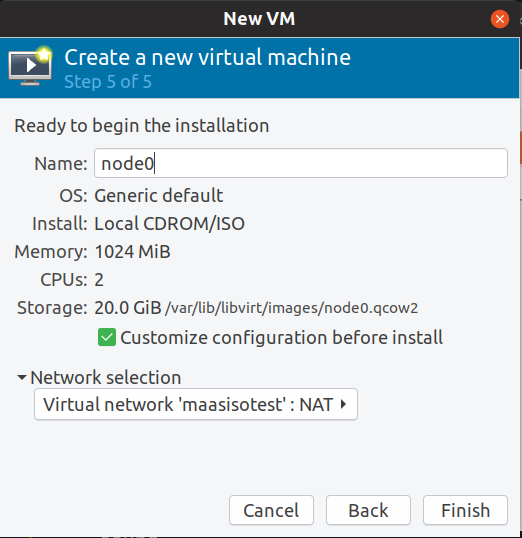
\includegraphics[width=0.5\textwidth]{images/5-1.png}
    \caption{Node 0}
\end{figure}


\begin{figure}[!ht]
    \centering
    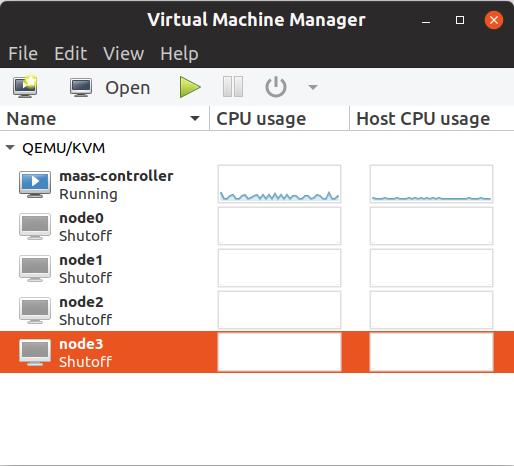
\includegraphics[width=0.5\textwidth]{images/5-2.png}
    \caption{Clones of node 0}
\end{figure}


Begin the installation and once the machine is open, pull the virtual power plug by force off, to create a few virtual machine clones.

Once the clones are created, power on all the virtual machines. These machines will boot for enlistment procedure. They will register themselves and shut themselves down.

\begin{figure}[!ht]
    \centering
    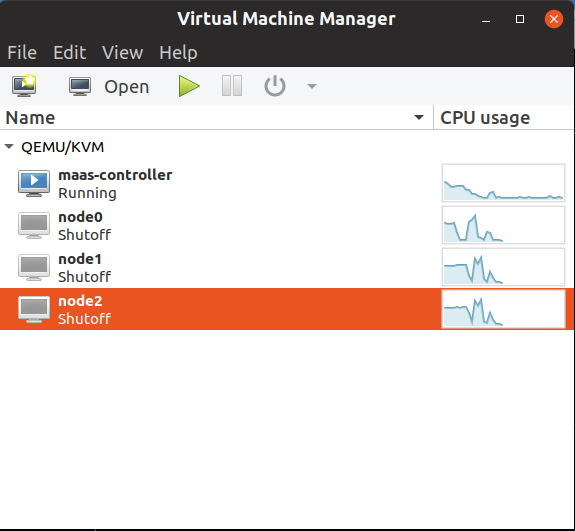
\includegraphics[width=0.5\textwidth]{images/5-3.png}
    \caption{Nodes enlisted themselves and shutdown}
\end{figure}

As soon as they shutdown, we will start confiiguring the power parameters. Before we do that, we need to change the identifications names of the nodes in the maas interface. To do this run the following command in the host:

\$ virsh dumpxml node0 | grep mac 

And then check for the device which has the same mac address in the maas interface and then set the name to node0. In the same way do for the other clones.

\begin{figure}[!ht]
    \centering
    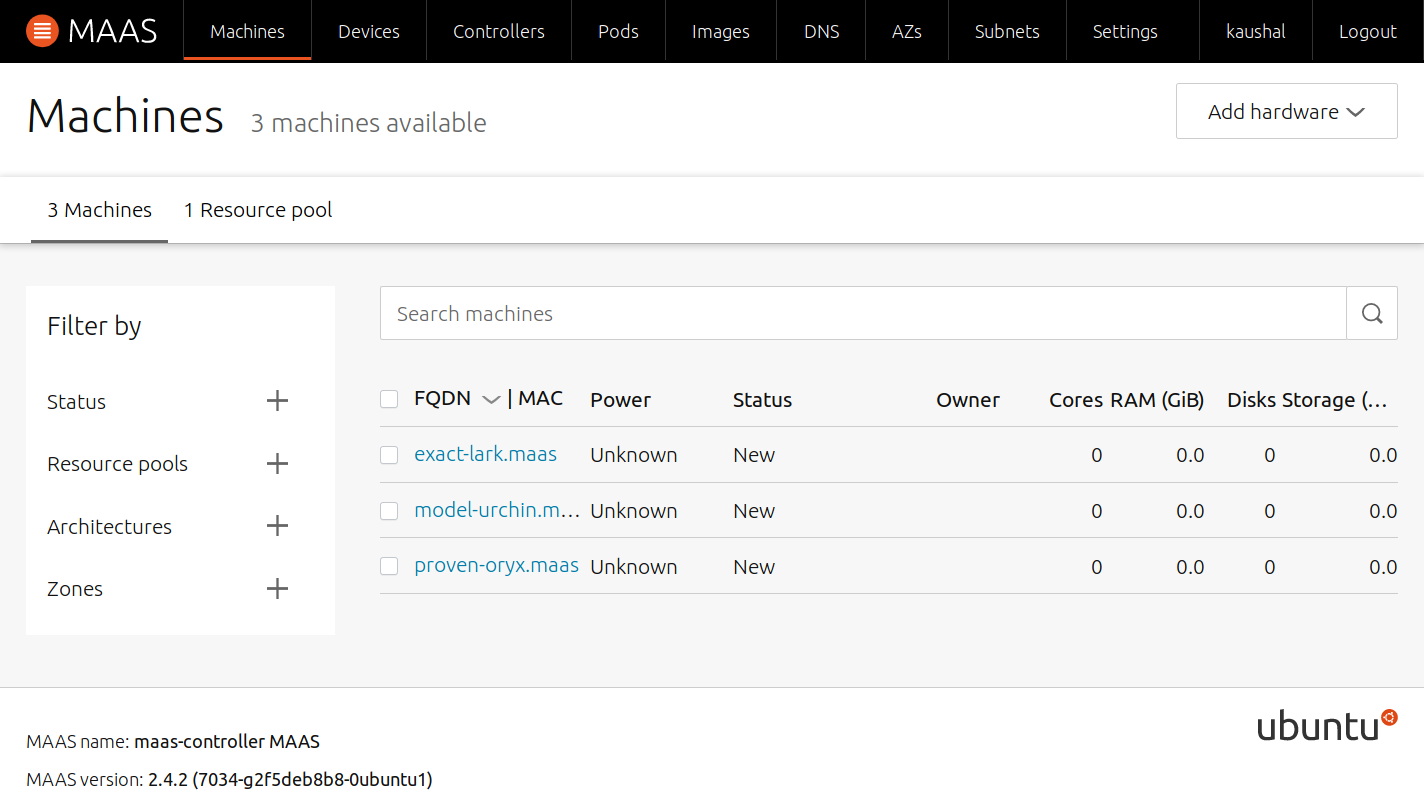
\includegraphics[width=0.7\textwidth]{images/5-4.png}
    \caption{Change these names to the meaningful names}
\end{figure}

Refer the Fig. 5.5 for power configuration of node0, likewise you need to configure power parameters for other nodes.

Power type: Virsh

Virsh Address: \url{qemu+ssh://kaushal@10.128.0.132/system}

Virsh VM ID: \url{node0}

\begin{figure}[!ht]
    \centering
    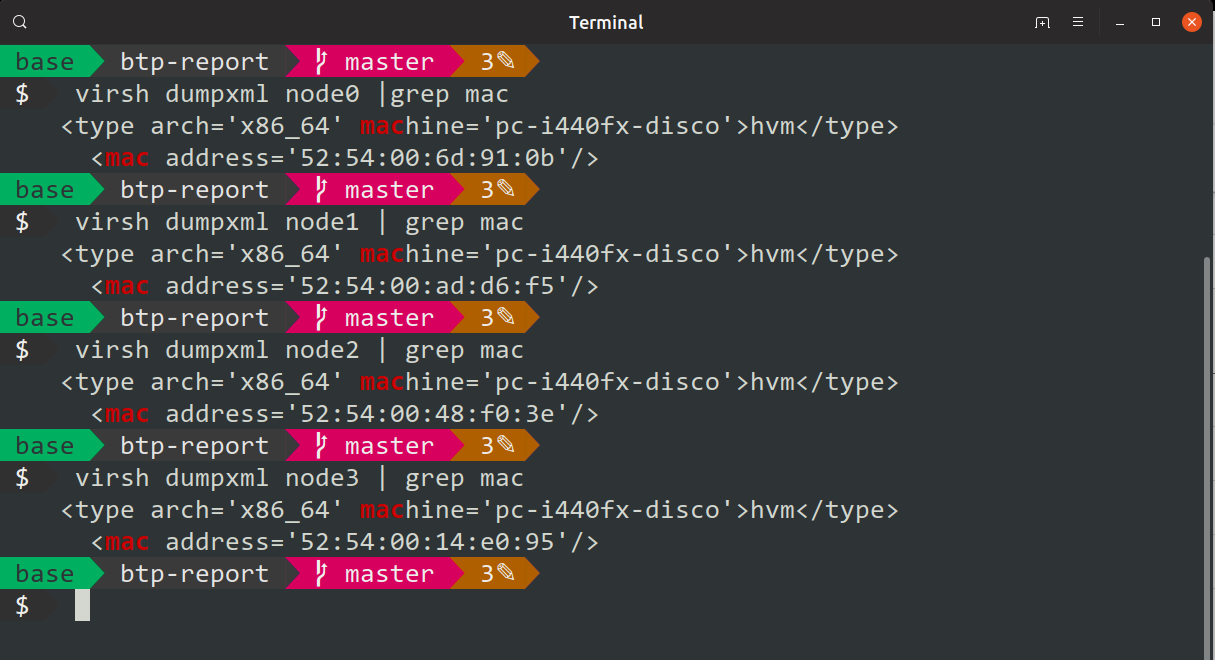
\includegraphics[width=0.7\textwidth]{images/5-5.png}
    \caption{Power configuration for node0}
\end{figure}

Once the power configuration is done select all nodes and commission all of them.

This is a basic procedure of how to create MAAS nodes and commission them.
\cleardoublepage 
\typeout{}
\chapname = {Future Work}

\chapter{Future Work}

Till now whatever we have done was in virtual environment but the actual aim of this project is to develop an experimental cloud using commodity hardware. In the next semester we will have to repeat the similar procedure for the commodity hardware. First step is to repurpose those hardwares according to our needs. Once that is done we will move on to setup similar environment.
\typeout{}

\bibliographystyle{IEEEtran}
\bibliography{btp}
\end{document}

